\subsection{Agent Function Architecture}\label{subsec:AgentFNArch}
\note{This section shows how the agent function is implemented. Diagram shows how DerivedOccupancyGridAgent actually operates.}
Putting together the components outlined so far in this chapter, we end up with an agent function that is shown in Figure \ref{fig:BasicAgentArchitecture}. 

\note{Fix this figure}
\begin{figure}
    \centering
    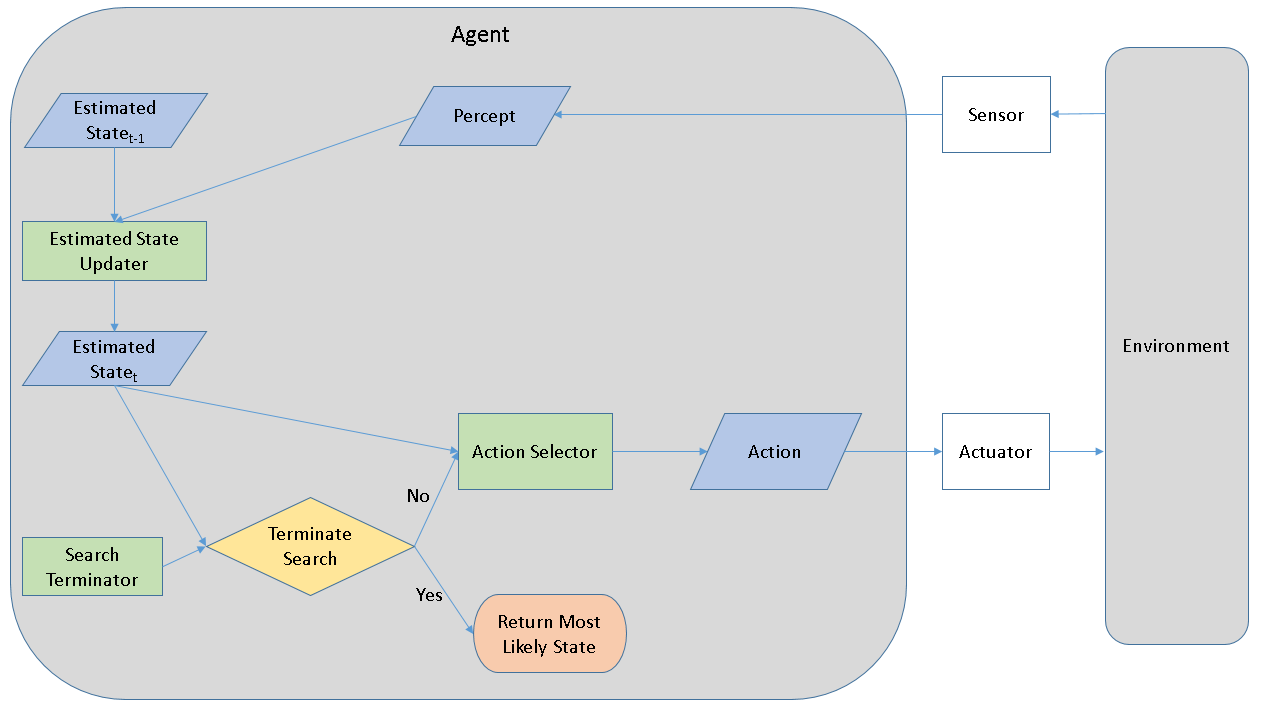
\includegraphics[width = 0.75\linewidth]{Chapters/MultiAgentTargetDetection/Figs/AgentFnArchitecture/BasicAgentFunctionNoCommunication.PNG}
    \caption{The structure of the agent function.}
    \label{fig:BasicAgentArchitecture}
\end{figure}


The diagram outlines how the agent interacts with its environment and abstracts away technical details such as the search status. This is a concrete version of the model-based reflex agent outlined in \cite[P~.51]{AIAMA}. The estimated state update rules are applied as outlined in the previous sections in this chapter.
\note{might be able to bulk this up a bit, come back to it}